\section{پروژه سوم: تخمین سن با یادگیری انتقالی (\lr{Transfer Learning})}

در این پروژه هدف ما طراحی و آموزش یک شبکه‌ی عصبی برای تخمین سن افراد از روی تصویر چهره است. با توجه به پیچیدگی استخراج ویژگی‌های چهره در سنین مختلف، به‌جای آموزش یک مدل از پایه، از تکنیک یادگیری انتقالی و معماری ازپیش‌آموزش‌دیده‌ی \lr{MobileNet} در فریم‌ورک \lr{Keras} استفاده کردیم. 

\vspace{0.4cm}
\subsection{آماده‌سازی مجموعه داده و استخراج برچسب‌ها}

برای این مسئله از مجموعه‌داده‌ی \lr{UTKFace} استفاده شده است. یکی از ویژگی‌های جالب این دیتاست، عدم وجود یک فایل جداگانه برای برچسب‌هاست؛ در واقع اطلاعات هر شخص (سن، جنسیت و نژاد) در نام فایل تصویر نهفته است. به عنوان مثال در فایلی با نام \lr{100\_1\_0\_...}، عدد اول (۱۰۰) نمایانگر سن شخص می‌باشد. 
ما با استفاده از یک اسکریپت پایتون، دیتاست را پیمایش کرده و سن هر شخص را از نام فایل استخراج کرده و به همراه مسیر تصویر، در یک دیتافریم ذخیره نمودیم.

\begin{stepbox}
\field{نرمال‌سازی و بالانس کردن توزیع سنی}{
با بررسی توزیع اولیه‌ی داده‌ها متوجه شدیم که توزیع تصاویر در سنین مختلف یکنواخت نیست. به‌خصوص تعداد تصاویر مربوط به نوزادان و کودکان زیر ۴ سال بسیار بیشتر از سایر بازه‌های سنی بود. این عدم تعادل می‌تواند باعث سوگیری (\lr{Bias}) مدل به سمت سنین پایین شود.

برای رفع این مشکل، میانگین تعداد نمونه‌ها در هر سن را محاسبه کرده و تصاویری که مربوط به سنین ۰ تا ۴ سال بودند و تعدادشان از این میانگین فراتر بود را با روش \lr{Down-sampling} کاهش دادیم تا توزیع داده‌ها به یک حالت نرمال‌تر و منطقی‌تر برسد.
}
\end{stepbox}

\begin{figure}[h!]
    \centering
    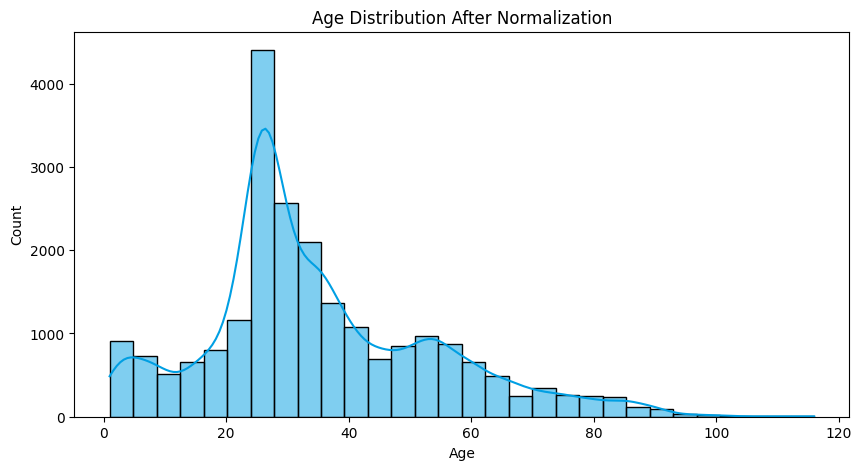
\includegraphics[width=0.85\textwidth]{images/age_distribution.png}
    \caption{توزیع سنی داده‌ها پس از اعمال نرمال‌سازی بر روی سنین زیر ۴ سال}
    \label{fig:age_distribution}
\end{figure}

\begin{notebox}[تحلیل توزیع سنی داده‌ها]
همان‌طور که در شکل \ref{fig:age_distribution} مشاهده می‌شود، با وجود اعمال نرمال‌سازی و کاهش هدفمند تصاویر سنین زیر ۴ سال، توزیع مجموعه‌داده همچنان کاملاً یکنواخت نیست. 

قله‌ی اصلی (بیشترین تراکم داده‌ها) در بازه‌ی سنی ۲۰ تا ۳۰ سال قرار دارد که تعداد آن‌ها به بیش از ۴۰۰۰ نمونه در یک سن خاص می‌رسد. این توزیعِ نرمال‌نشده‌ی ذاتی در دیتاست، به این معناست که شبکه‌ی ما احتمالاً در تخمین سن افراد جوان (۲۰ تا ۳۰ سال) عملکرد بسیار دقیق‌تری خواهد داشت، اما ممکن است برای سنین بالاتر (به‌ویژه بالای ۶۰ سال) به دلیل کمبود نسبی داده‌ی آموزشی، با خطای بیشتری مواجه شود. با این حال، کاهش اولیه‌ی داده‌های سنین نوزادی، از یک سوگیری (\lr{Bias}) شدید و مخرب به سمت سنین صفر تا چهار سال جلوگیری کرده است.
\end{notebox}

پس از متوازن‌سازی، مجموعه‌داده‌ی نهایی به سه بخش آموزش (\lr{Train})، اعتبارسنجی (\lr{Validation}) و آزمون (\lr{Test}) با نسبت‌های استاندارد تقسیم شد تا مدل در مراحل بعدی روی آن‌ها آموزش دیده و ارزیابی گردد.

\vspace{0.4cm}
\subsection{معماری شبکه و طراحی مدل یادگیری انتقالی}

برای تخمین سن (که در اینجا به عنوان یک مسئله‌ی رگرسیون مدل‌سازی شده است)، استفاده از مدل‌های ازپیش‌آموزش‌دیده گزینه‌ی بسیار مناسبی است. ما از معماری \lr{MobileNet} که روی مجموعه‌داده‌ی \lr{ImageNet} آموزش دیده است، به عنوان پایه‌ی استخراج ویژگی استفاده کردیم.

\begin{stepbox}
\field{پیکربندی لایه‌ها و استراتژی آموزش}{
\begin{itemize}
    \item \textbf{ورودی و پیش‌پردازش:} تصاویر به ابعاد $128 \times 128$ پیکسل تغییر اندازه داده شده و با تابع \lr{preprocess\_input} مختص \lr{MobileNet} نرمال‌سازی شدند. جهت مدیریت بهینه‌ی حافظه (\lr{RAM}) در محیط \lr{Colab}، از خط لوله‌ی \lr{tf.data} با اندازه‌ی دسته‌ی (\lr{Batch Size}) برابر با ۱۶ استفاده گردید.
    \item \textbf{فریز کردن لایه‌های پایه (\lr{Feature Extraction}):} در فاز نخست، تمامی لایه‌های کانولوشنی \lr{MobileNet} فریز شدند (\lr{Trainable = False}). این کار باعث می‌شود وزن‌های ازپیش‌آموزش‌دیده‌ی شبکه‌ی پایه حفظ شوند. همان‌طور که در خلاصه‌ی مدل (\lr{Model Summary}) مشخص است، از حدود ۳.۳ میلیون پارامتر مدل، تنها ۱۳۱ هزار پارامتر قابل آموزش (\lr{Trainable}) هستند.
    \item \textbf{طراحی سر شبکه (\lr{Custom Head}):} پس از لایه‌ی تجمیع سراسری (\lr{GlobalAveragePooling2D})، یک لایه‌ی متراکم ۱۲۸ نودی (\lr{ReLU}) و یک لایه‌ی \lr{Dropout} با نرخ $0.3$ قرار گرفت. لایه‌ی خروجی شامل یک نورون با فعال‌ساز خطی (\lr{Linear}) برای تخمین مقدار پیوسته‌ی سن است.
\end{itemize}
}
\end{stepbox}

\vspace{0.3cm}
\begin{notebox}[تحلیل نتایج فاز اول آموزش]
مدل در فاز اول با استفاده از تابع زیان میانگین خطای مطلق (\lr{MAE}) و بهینه‌ساز \lr{Adam} با نرخ یادگیری $0.001$، به مدت ۱۰ اپوک آموزش دید. برای اطمینان از ذخیره‌ی بهترین نتایج، از \lr{ModelCheckpoint} استفاده شد. 

در پایان این مرحله، خطای اعتبارسنجی (\lr{val\_mae}) به عدد \textbf{$7.72$ سال} کاهش یافت. این بدان معناست که مدل با وجود فریز بودن تمام لایه‌های اصلی استخراج ویژگی، توانسته است خطای تخمین سن را به‌طور میانگین به کمتر از ۸ سال برساند. این عملکرد اولیه بسیار امیدوارکننده است، اما برای بهبود بیشتر نیازمند تنظیم دقیق (\lr{Fine-Tuning}) لایه‌های پایه هستیم.
\end{notebox}

\vspace{0.4cm}

\subsection{فاز دوم آموزش: تنظیم دقیق (\lr{Fine-Tuning})}

پس از همگرایی نسبی لایه‌ی خروجی در فاز اول، برای افزایش دقت تخمین مدل و یادگیری ویژگی‌های ظریف‌تر چهره (نظیر خطوط چهره و تغییرات بافت پوست در سنین مختلف)، تمامی لایه‌های شبکه‌ی \lr{MobileNet} را از حالت فریز خارج کردیم (\lr{Trainable = True}).

\begin{stepbox}
\field{استراتژی تنظیم دقیق}{
\begin{itemize}
    \item \textbf{نرخ یادگیری بسیار کوچک:} برای جلوگیری از تخریب وزن‌های ازپیش‌آموزش‌دیده‌ی شبکه‌ی پایه (پدیده‌ی \lr{Catastrophic Forgetting})، مدل را با بهینه‌ساز \lr{Adam} و نرخ یادگیری بسیار پایینِ $10^{-5}$ مجدداً کامپایل کردیم.
    \item \textbf{آموزش سراسری:} در این مرحله تمامی ۳.۳ میلیون پارامتر مدل در فرآیند به‌روزرسانی وزن‌ها شرکت داشتند و مدل برای ۱۰ اپوک دیگر آموزش دید.
\end{itemize}
}
\end{stepbox}

\begin{figure}[h!]
    \centering
    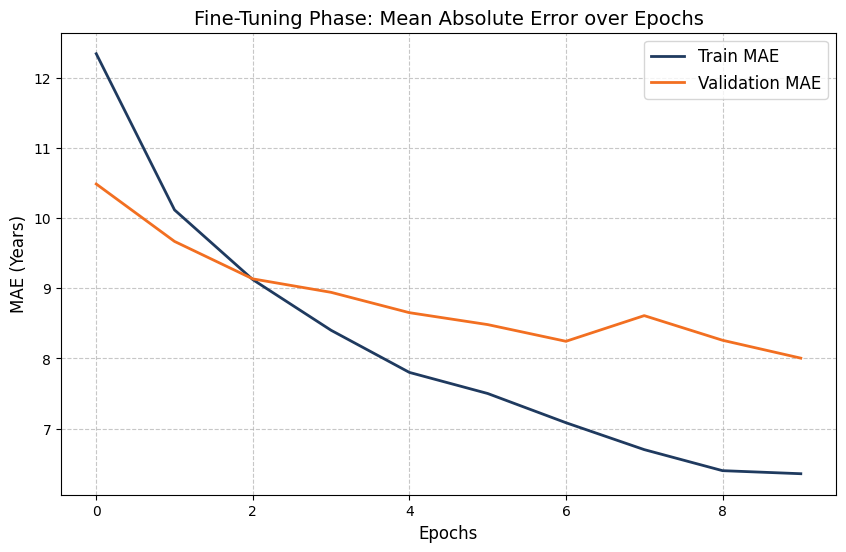
\includegraphics[width=0.85\textwidth]{images/finetuning_history.png}
    \caption{روند کاهش میانگین خطای مطلق (\lr{MAE}) در فاز تنظیم دقیق برای داده‌های آموزش و اعتبارسنجی}
    \label{fig:finetuning_history}
\end{figure}

\begin{notebox}[تحلیل عملکرد در فاز تنظیم دقیق]
همان‌طور که در نمودار شکل \ref{fig:finetuning_history} مشخص است، با باز شدن لایه‌های پایه، مدل توانست الگوهای بهتری را استخراج کند. خطای آموزش به حدود $6.35$ سال رسید و خطای اعتبارسنجی نیز تا $8.00$ سال کاهش یافت. 
نوسانات موجود در نمودار اعتبارسنجی و فاصله‌گرفتن آن از خطای آموزش در اپوک‌های پایانی، نشان‌دهنده‌ی شروع پدیده‌ی بیش‌برازش (\lr{Overfitting}) است؛ اما استفاده از \lr{ModelCheckpoint} تضمین کرد که وزن‌های مربوط به کمترین خطای اعتبارسنجی (اپوک دهم) برای ارزیابی نهایی ذخیره شوند.
\end{notebox}


\vspace{0.4cm}
\subsection{بهینه‌سازی هایپرپارامترها و تنظیم دقیق (\lr{Fine-Tuning})}

پس از همگرایی نسبی لایه‌ی خروجی در فاز اول، تصمیم گرفتیم برای یادگیری ویژگی‌های ظریف‌تر چهره، تمامی لایه‌های شبکه‌ی \lr{MobileNet} را از حالت فریز خارج کنیم (\lr{Trainable = True}). با ارزیابی‌های اولیه متوجه شدیم که مدل دچار کم‌برازش (\lr{Underfitting}) روی الگوهای پیچیده‌ی سنی است. برخلاف تجربه‌ی کار با فریم‌ورک پایتورچ برای پروژه‌ی تشخیص احساسات چهره که در آن الگوهای گذرا و حالت عضلات صورت اهمیت بالایی داشتند، در این پروژه شبکه‌ی ما نیازمند درک دقیق بافت دائمی پوست و چین‌وچروک‌ها بود.

برای رفع محدودیت‌های مدل و افزایش دقت، تغییرات زیر در خط لوله‌ی پردازش و آموزش اعمال گردید:

\newpage
\begin{stepbox}
\field{اصلاح ابعاد ورودی و متغیرهای آموزش}{
\begin{itemize}
    \item \textbf{حفظ رزولوشن اصلی تصاویر:} تغییر ابعاد تصاویر به $128 \times 128$ باعث از بین رفتن بافت‌های ظریف و روتوش شدن چهره‌ها شده بود که منجر به پیش‌بینی سنین بسیار پایین‌تر می‌گردید. با بازگرداندن ابعاد به اندازه‌ی اصلی دیتاست ($200 \times 200$)، این مشکل برطرف شد.
    \item \textbf{افزایش نرخ \lr{Dropout}:} نرخ لایه‌ی \lr{Dropout} از $0.3$ به $0.5$ افزایش یافت تا شبکه به جای تکیه بر ویژگی‌های خاص، ساختار کلی چهره را درک کند.
    \item \textbf{نرخ یادگیری و طول آموزش:} نرخ یادگیری در فاز دوم روی $3 \times 10^{-5}$ تنظیم شد و تعداد اپوک‌ها به ۳۰ ارتقا یافت تا مدل فرصت کافی برای تطبیق با جزئیات جدید را داشته باشد.
\end{itemize}
}
\end{stepbox}

\begin{figure}[h!]
    \centering
    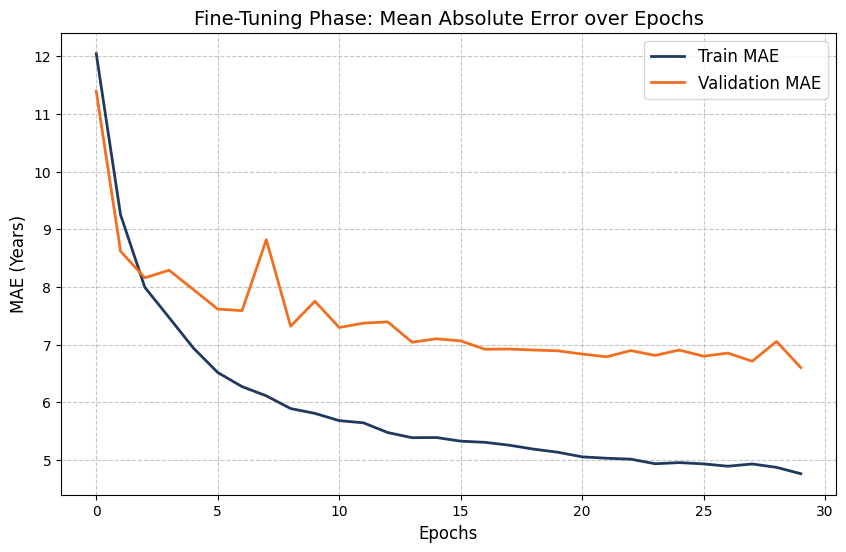
\includegraphics[width=0.85\textwidth]{images/finetuning_history_2.png}
    \caption{روند کاهش میانگین خطای مطلق (\lr{MAE}) در فاز تنظیم دقیق پس از اعمال بهینه‌سازی‌ها}
    \label{fig:finetuning_history}
\end{figure}

همان‌طور که در نمودار شکل \ref{fig:finetuning_history} مشخص است، مدل توانست الگوهای بهتری را استخراج کند و خطای اعتبارسنجی با روندی نزولی و منطقی کاهش یابد. استفاده از \lr{ModelCheckpoint} نیز تضمین کرد که بهترین وزن‌های شبکه در طول این ۳۰ اپوک برای ارزیابی نهایی ذخیره شوند.

\vspace{0.4cm}
\subsection{ارزیابی نهایی و تست در شرایط واقعی (\lr{Inference})}

در گام نهایی، بهترین وزن‌های ذخیره‌شده‌ی مدل بارگذاری گردید و عملکرد شبکه بر روی مجموعه‌داده‌ی آزمون (\lr{Test Dataset}) ارزیابی شد. به لطف بهینه‌سازی‌های انجام شده، خطای میانگین مطلق (\lr{MAE}) روی داده‌های آزمون به عدد بسیار مطلوب \textbf{$6.66$ سال} رسید.

برای درک بهتر عملکرد شبکه در محیط عملیاتی، مدل را بر روی چند تصویر تصادفی از مجموعه‌ی آزمون اعمال کردیم (شکل \ref{fig:inference_results}).

\begin{figure}[h!]
    \centering
    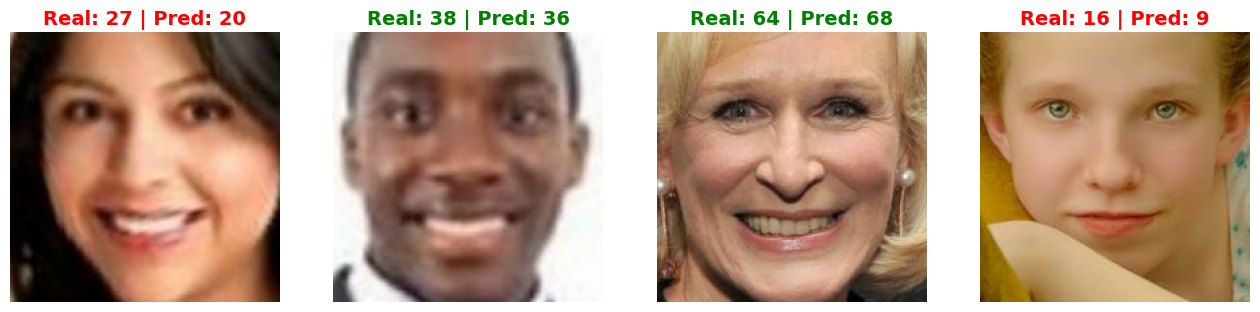
\includegraphics[width=0.95\textwidth]{images/inference_results.png}
    \caption{نمونه‌هایی از خروجی نهایی مدل روی داده‌های آزمون. سن واقعی (\lr{Real}) و سن پیش‌بینی‌شده (\lr{Pred}) مشخص شده‌اند.}
    \label{fig:inference_results}
\end{figure}

\begin{tipbox}[جمع‌بندی عملکرد مدل]
نتایج بصری نشان می‌دهند که مدل بهبود یافته‌ی ما توانایی بالایی در تشخیص سن افراد میانسال و مسن پیدا کرده است (مانند پیش‌بینی ۳۶ سال برای فرد ۳۸ ساله و ۶۸ سال برای فرد ۶۴ ساله که با رنگ سبز مشخص شده‌اند). خطاهای باقیمانده عمدتاً مربوط به تفاوت سن بیولوژیکی با ظاهر افراد، شرایط نوری، یا زاویه‌ی دید دوربین است که با توجه به چالش‌های ذاتی مسئله‌ی تخمین سن، عملکرد شبکه کاملاً موفقیت‌آمیز ارزیابی می‌شود.
\end{tipbox}